\documentclass[page number]{beamer}
\usepackage{etex}
\usepackage{graphicx, booktabs} % For tabulars
\usepackage{pgf,tikz}
\usepackage{ulem}
\usetikzlibrary{arrows}
\usetikzlibrary{positioning,shapes,fit}
\usepackage{algorithm}
\usepackage{algpseudocode}
\usepackage{multicol}
\usepackage{syntax}
\usepackage{xcolor, color, colortbl}
\usepackage{tikz-qtree}
\usepackage{listings}

\setbeamertemplate{navigation symbols}{}
\beamertemplatenavigationsymbolsempty% remove navigation bar

\definecolor{basicBlue}{HTML}{297FB8} % #297FB8
\definecolor{basicCyan}{HTML}{16A086} % #16A086
\definecolor{basicGreen}{HTML}{9BBB58} % #9BBB58
\definecolor{basicRed}{HTML}{C1392B} % #C1392B
\definecolor{basicPurple}{HTML}{7A0333} % #7A0333

\colorlet{darkBlue}{basicBlue!70!black}
\colorlet{darkCyan}{basicCyan!80!black}
\colorlet{darkGreen}{basicGreen!80!black}

\setbeamercolor{titlelike}{fg=darkBlue}
\setbeamercolor{separation line}{fg=basicGreen}
\setbeamercolor{local structure}{fg=basicBlue}
\setbeamercolor{section in toc}{fg=darkBlue}
\setbeamercolor{block title}{fg=darkCyan!60!black, bg=darkCyan!20}
\setbeamercolor{block body}{bg=darkCyan!10}
\setbeamercolor{block title example}{fg=darkGreen!60!black, bg=darkGreen!20}
\setbeamercolor{block body example}{bg=darkGreen!10}
\setbeamercolor{block title alerted}{fg=basicRed!50!black, bg=basicRed!20}
\setbeamercolor{block body alerted}{bg=basicRed!10}
\setbeamercolor{section in head/foot}{bg=basicBlue!60!black, fg=white}




\newcommand{\HRule}[1]{\rule{\linewidth}{#1}}

\setbeamertemplate{headline}{
  \begin{beamercolorbox}[ht=12pt]{section in head/foot}
    \insertsectionnavigationhorizontal{.5\textwidth}{\hskip5pt }{}
    \vspace{2pt}
  \end{beamercolorbox}%
}

\setbeamertemplate{footline}{

  \begin{beamercolorbox}[ht=10pt]{section in head/foot}

      \raisebox{2pt}[0pt][0pt] {
        \makebox[0.5\textwidth][l]{\hskip10pt \insertshorttitle}%
        \makebox[0.5\textwidth][r]{\insertframenumber/ \inserttotalframenumber \hskip10pt }%
      }
  \end{beamercolorbox}%
  % \hfill\color{basicBlue}
  % \makebox[20pt][c]{%
  %   \raisebox{5pt}[0pt][0pt] {%
  %   }
  % }
}

\setbeamertemplate{title page} {
  \begin{center}
    {
    \color{basicBlue}
    \HRule{0.5pt} \\
    \vspace{2pt}
    { \Large \color{darkBlue}
    \textsc{\usebeamerfont{title}\usebeamercolor[fg]{title}\inserttitle}}
    \HRule{2pt} \\
    }
    \vspace{10pt}

    {\footnotesize
    \begin{minipage}[t]{0.4\textwidth}
    \begin{flushleft}
    {\it \color{darkCyan}Author:}\\
    \color{darkBlue}Aur\`ele \textsc{Barri\`ere}
    \end{flushleft}
    \end{minipage}
    \begin{minipage}[t]{0.4\textwidth}
    \begin{flushright}
    {\it \color{darkCyan}Supervisors:}\\
    \color{darkBlue}Prof. Chung-Kil \textsc{Hur}\\
    \color{darkBlue}Jeehoon \textsc{Kang}
    \end{flushright}
    \end{minipage}\\
    }
  { \color{darkCyan}
    \vspace{10pt}
  \insertdate%
  }
  \end{center}
}

  \newsavebox{\contentbox}
  \newlength{\heightBox}


\newcommand{\lightenv}[2]{
  \savebox{\contentbox}{
  \begin{minipage}{0.8\textwidth}
    \vspace{5pt}
  #2
    \vspace{5pt}
  \end{minipage}
  }
  \setlength{\heightBox}{\dimexpr\ht\contentbox+\dp\contentbox}
  {\setlength\tabcolsep{2pt}
  \begin{tabular}{l c}
    {\begin{minipage}{4pt}
      \centering%
      \begin{tikzpicture}%
        \draw[line width=4pt,line cap=butt,color=#1] (0,\heightBox)--(0,0);
      \end{tikzpicture}%
    \end{minipage}}%
    &
    \usebox{\contentbox}%
  \end{tabular}
  }
}


\makeatletter

%  http://tex.stackexchange.com/questions/46434/how-to-highlight-text-formals-with-tikz
\makeatletter
%
% Highlighter code
%

\tikzset{%
  remember picture with id/.style={%
    remember picture,
    overlay,
    save picture id=#1,
  },
  save picture id/.code={%
    \edef\pgf@temp{#1}%
    \immediate\write\pgfutil@auxout{%
      \noexpand\savepointas{\pgf@temp}{\pgfpictureid}}%
  }
}

\def\savepointas#1#2{%
  \expandafter\gdef\csname save@pt@#1\endcsname{#2}%
}

\tikzdeclarecoordinatesystem{pic}{%
  \@ifundefined{save@pt@#1}{%
    \pgfpointorigin
  }{%
  \pgfsys@getposition{\csname save@pt@#1\endcsname}\save@orig@pic%
  \pgfsys@getposition{\pgfpictureid}\save@this@pic%
  \pgf@process{\pgfpointorigin\save@this@pic}%
  \pgf@xa=\pgf@x
  \pgf@ya=\pgf@y
  \pgf@process{\pgfpointorigin\save@orig@pic}%
  \advance\pgf@x by -\pgf@xa
  \advance\pgf@y by -\pgf@ya
  }%
}

\newcounter{highlight}
\newcommand{\hlstart}{\tikz[remember picture with id=hlstart\the\value{highlight},baseline=-0.7ex];\hl@start}
\newcommand{\hlend}{\tikz[remember picture with id=hlend\the\value{highlight},baseline=-0.7ex];\hl@end\stepcounter{highlight}}
\newcommand{\fdstart}{\tikz[remember picture with id=hlstart\the\value{highlight},baseline=-0.7ex];\fd@start}
\newcommand{\fdend}{\tikz[remember picture with id=hlend\the\value{highlight},baseline=-0.7ex];\fd@end\stepcounter{highlight}}
\newcommand{\vlstart}{\tikz[remember picture with id=hlstart\the\value{highlight},baseline=-1em];\vl@start}
\newcommand{\vlend}{\tikz[remember picture with id=hlend\the\value{highlight},baseline=0.3ex];\vl@end\stepcounter{highlight}}

\newcommand{\hl@start}[1][]{%
  \hl@draw{highlighter}{#1}{\the\value{highlight}}}

\newcommand{\hl@end}{}

\newcommand{\fd@start}[1][]{%
  \def\fd@args{#1}}

\newcommand{\fd@end}{\def\@tempa{\hl@draw{fader}}\expandafter\@tempa\expandafter{\fd@args}{\the\value{highlight}}\def\fd@args{}}

\newcommand{\vl@start}[1][]{%
  \vl@draw{highlighter}{#1}{\the\value{highlight}}}

\newcommand{\vl@end}{}


\def\hl@sets{%
  \edef\hl@sx{\the\pgf@x}%
  \edef\hl@sy{\the\pgf@y}%
}
\def\hl@sete{%
  \edef\hl@ex{\the\pgf@x}%
  \edef\hl@ey{\the\pgf@y}%
}

\@ifclassloaded{beamer}{

\def\page@node{
  \path (current page.south east)
      ++(-\beamer@rightmargin,\footheight)
  node[
    minimum width=\textwidth,
    minimum height=\textheight,
    anchor=south east
  ] (page) {};
}

}{

  \def\page@node{
    \path (current page.north west)
    ++(\hoffset + 1in + \oddsidemargin + \leftskip,\voffset + 1in + \topmargin + \headheight + \headsep)
    node[
      minimum width=\textwidth - \leftskip - \rightskip,
      minimum height=\textheight,
      anchor=north west
    ] (page) {};
  }

}

\newcommand{\hl@draw}[3]{%
  \begin{tikzpicture}[remember picture,overlay]%
  \page@node
  \tikzset{#2,highlight=#1,every path/.append style={highlight=#1}}%
  \pgfmathsetlengthmacro{\hl@width}{\the\pgflinewidth - 1pt}%
  \coordinate (hlstart) at (pic cs:hlstart#3);
  \coordinate (hlend) at (pic cs:hlend#3);
  \tikz@scan@one@point\hl@sets(pic cs:hlstart#3)
  \tikz@scan@one@point\hl@sete(pic cs:hlend#3)
  \ifdim\hl@sy=\hl@ey\relax
  \draw (hlstart) -- (hlend);
  \else
  \draw (hlstart) -- (hlstart -| page.east);
  \pgfmathsetlengthmacro{\hl@sy}{\hl@sy -\hl@width}%
  \pgfmathsetlengthmacro{\hl@ey}{\hl@ey +\hl@width}%
  \loop\ifdim\hl@sy>\hl@ey\relax
  \draw (0,\hl@sy -| page.west) -- (0,\hl@sy -| page.east);
  \pgfmathsetlengthmacro{\hl@sy}{\hl@sy -\hl@width}%
  \repeat
  \draw (hlend -| page.west) -- (hlend);
  \fi
  \end{tikzpicture}%
}

\newcommand{\vl@draw}[3]{%
  \begin{tikzpicture}[remember picture,overlay]%
  \page@node
  \tikzset{#2,highlight=#1,every path/.append style={highlight=#1}}%
  \pgfmathsetlengthmacro{\hl@width}{\the\pgflinewidth - 1pt}%
  \coordinate (hlstart) at (pic cs:hlstart#3);
  \coordinate (hlend) at (pic cs:hlend#3);
  \tikz@scan@one@point\hl@sets(pic cs:hlstart#3)
  \tikz@scan@one@point\hl@sete(pic cs:hlend#3)
  \ifdim\hl@sx=\hl@ex\relax
  \draw (hlstart) -- (hlend);
  \else
  \draw (hlstart) -- (hlstart |- page.south);
  \pgfmathsetlengthmacro{\hl@sx}{\hl@sx -\hl@width}%
  \pgfmathsetlengthmacro{\hl@ex}{\hl@ex +\hl@width}%
  \loop\ifdim\hl@sx>\hl@ex\relax
  \draw (\hl@sx,0 |- page.north) -- (\hl@sx,0 |- page.south);
  \pgfmathsetlengthmacro{\hl@sx}{\hl@sx -\hl@width}%
  \repeat
  \draw (hlend |- page.north) -- (hlend);
  \fi
  \end{tikzpicture}%
}

\tikzset{%
  highlight/.default=highlighter,
  highlight/.style={
    color=\pgfkeysvalueof{/tikz/#1 colour},
    line width=\pgfkeysvalueof{/tikz/#1 width},
    line cap=\pgfkeysvalueof{/tikz/#1 cap},
    opacity=\pgfkeysvalueof{/tikz/#1 opacity},
  },
  highlighter colour/.initial=yellow,
  highlighter width/.initial=14pt,% <-- Tweak (was 12pt)
  highlighter cap/.initial=butt,
  highlighter opacity/.initial=1,
  fader colour/.initial=gray,
  fader width/.initial=12pt,
  fader cap/.initial=butt,
  fader opacity/.initial=.5,
}



\@ifclassloaded{beamer}{

%% Beamer variants

\setbeamercolor{highlighted text}{bg=yellow}
\setbeamercolor{faded text}{fg=gray}

\newcommand<>{\highlight}[2][]{%
  \only#3{\hlstart[#1]}#2\only#3{\hlend}}

\newcommand<>{\fade}[2][]{%
  \only#3{\fdstart[#1]}#2\only#3{\fdend}}

\newcommand<>{\vhighlight}[2][]{%
  \only#3{\vlstart[#1]}#2\only#3{\vlend}}

}{

\newcommand{\highlight}[2][]{%
\hlstart[#1]#2\hlend}

\newcommand{\fade}[2][]{%
\fdstart[#1]#2\fdend}

\newcommand{\vhighlight}[2][]{%
\vlstart[#1]#2\vlend}

}


\newcommand{\diam}[1]{\!<\!\!#1\!\!>\!}

\newcommand{\dlenv}[1]{\lightenv{basicGreen}{#1}}
\newcommand{\slenv}[1]{\lightenv{basicCyan}{#1}}


\makeatother

\setcounter{tocdepth}{1} % remove subsection from table of contents

%counting frames
\newcommand{\backupbegin}{
   \newcounter{framenumberappendix}
   \setcounter{framenumberappendix}{\value{framenumber}}
}
\newcommand{\backupend}{
   \addtocounter{framenumberappendix}{-\value{framenumber}}
   \addtocounter{framenumber}{\value{framenumberappendix}}
}


\begin{document}
\title[Int-Ptr casts in CompCert]{Implementing a memory model supporting int-ptr casts in CompCert}


\author{Aur\`ele Barri\`ere}

\def\todo#1{{\color{red}TODO:\quad#1}}
\def\addref#1{{\color{red}$[$#1$]$}}
\def\undef{\textit{undef}}
\def\states#1{\mathit{States_{#1}}}
\def\step#1{\mathit{Step_{#1}}}
\def\atstep#1{\mathit{AtomicStep_{#1}}}
\def\traces{\mathit{Traces}}
\def\comment#1{{\color{blue}\textit{#1}}}
\def\outline{
  \begin{frame}
    \frametitle{Outline}
    \tableofcontents[currentsection]
  \end{frame}
}


\lstset{%
  basicstyle=\footnotesize,
  language=C,
  keywordstyle=\color{basicPurple}\textbf
  }


\begin{frame}[plain]
  \titlepage%
  \vfill
  \begin{center}
    
\includegraphics[width=2.5cm]{img/enslogo.png}
    \hfill
    
\includegraphics[width=2.5cm]{img/snulogo.png}
  \end{center}
\end{frame}

\section{Introduction}
\begin{frame}[fragile]{\secname : Integer-Pointer casting in C}

  \begin{minipage}{0.48\textwidth}
    \lstinputlisting{listings/intro.c}
  \end{minipage}
  \begin{minipage}{0.48\textwidth}
  \begin{alertblock}{ISO C Standard}
    \begin{itemize}
    \item Defines semantics for C programs.
    \item Undefined of unspecified behavior.
    \item \texttt{uintptr\_t}
    \end{itemize}
  \end{alertblock}
  \end{minipage}
  \vfill
  \begin{exampleblock}{Integer arithmetic on pointers has many uses}
    Linux Kernel, JVM implementations, FreeBSD\dots
  \end{exampleblock}
  
\end{frame}

\begin{frame}{Giving semantics to Integer-Pointer Casts in C}

  \begin{block}{Kang et al: A Formal C Memory Model Supporting Integer-Pointer Casts}
    \begin{itemize}
    \item Gives precise semantics to Int-Ptr casts.
    \item Allow common optimizations
    \end{itemize}
  \end{block}

\end{frame}


\begin{frame}{CompCert: a certified C compiler}

  \begin{block}{CompCert}
    \begin{itemize}
      \item From C to ASM (x86, powerpc or arm).
      \item Most passes are proved in Coq.
      \item Supports most of the ISO-C-99 standard.
    \end{itemize}
  \end{block}
  \vfill
  \begin{center}
    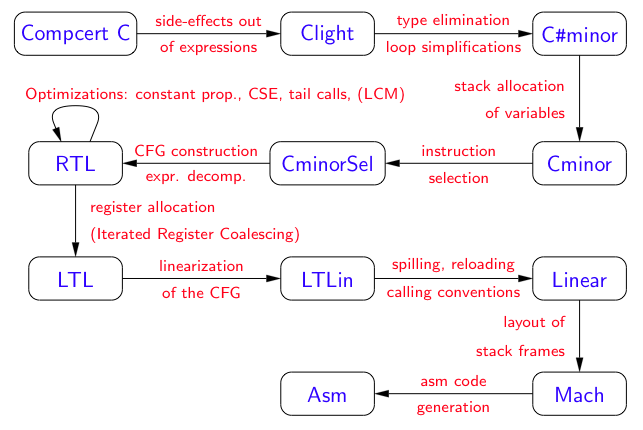
\includegraphics[scale=0.6]{img/passes.png}
  \end{center}
  
\end{frame}


\begin{frame}{Aim of this work}
  
  \begin{block}{Goals}
    \begin{itemize}
    \item Implement the new memory model in CompCert.
    \item Implement the Integer-Pointer cast semantics.
    \item Prove the correctness of compilation with this new model.
    \end{itemize}
  \end{block}
  \vfill
  \begin{exampleblock}{Benefits}
    \begin{itemize}
    \item Relevance and usability of the new memory model and semantics.
    \item Allow CompCert to compile correctly a bigger set of C programs.
    \end{itemize}
  \end{exampleblock}

\end{frame}


\section{C Memory Models}
\outline
\subsection{Logical Memory Model}
\begin{frame}{\subsecname}

  \begin{block}{Memory blocks}
    \begin{itemize}
    \item $\texttt{Block}=\{(v,n,c)~|~v\in\texttt{Bool},n\in\mathbb{N},c\in\texttt{Val}^{n}\}$
    \item Infinite memory.
    \item Optimizations.
    \end{itemize}
  \end{block}
  \vfill
  \begin{center}
    \begin{tabular}{l c r}
      \lstinputlisting[linewidth=3cm]{listings/logical.c} &
      $\xrightarrow[\text{Dead Alloc Elimination}]{\text{Constant Propagation}}$ &
      \lstinputlisting[linewidth=3cm]{listings/logicaloptim.c}
    \end{tabular}
  \end{center}
  \vfill
  \begin{alertblock}{No semantics for Integer-Pointer cast (unspecified)}
  \end{alertblock}
  
\end{frame}

\subsection{Concrete Memory Model}
\begin{frame}{\subsecname}

  \begin{block}{Memory blocks}
    Blocks are given a concrete address and a size.\\
    \textbf{Memory consistency:}
    \begin{itemize}
    \item Blocks should not overflow the finite memory.
    \item Blocks should not be overlapping.
    \end{itemize}
  \end{block}
  \vfill
  \begin{exampleblock}{Int-Ptr cast}
    Easy semantics for Integer-pointer casts.
  \end{exampleblock}
  \vfill
  \begin{alertblock}{No optimizations}
    A function can access any memory address.
  \end{alertblock}

\end{frame}

\subsection{Quasi-Concrete Memory Model}
\begin{frame}{\subsecname}

  \begin{block}{Memory blocks}
    \begin{itemize}
    \item $\texttt{Block}=\{(v,p,n,c)~|~v\in\texttt{Bool},n\in\mathbb{N},c\in\texttt{Val}^{n},$\\
      {\color{purple}$\mathbf{p\in\texttt{int32}\cup\{\undef\}}$}$\}$.
    \item Memory consistency (\textbf{No overflow}, \textbf{No overlap}) for concrete blocks.
    \end{itemize}
  \end{block}
  \vfill
  \begin{exampleblock}{Properties}
    \begin{itemize}
    \item Optimizations are possible with logical blocks.
    \item Integer-Pointer cast is possible with concrete blocks.
    \end{itemize}
  \end{exampleblock}
  
\end{frame}

\begin{frame}{The Capture Function}

  \begin{tabular}{l c r}
    \lstinputlisting[linewidth=4.3cm]{listings/capture.c} & $\longrightarrow$ &
    \lstinputlisting[linewidth=4.3cm]{listings/captured.c}
  \end{tabular}
  \vfill
  \begin{alertblock}{Non-determinism}
    A logical block can be captured at several different addresses.
  \end{alertblock}
  
\end{frame}

%\begin{frame}{Examples}
%  \begin{tabular}{l c r}
%    \lstinputlisting[linewidth=3cm]{listings/logical.c} &
%    $\xrightarrow[\text{Quasi-Concrete Model}]{\text{Logical Model}}$ & 
%    \lstinputlisting[linewidth=3.5cm]{listings/logicaloptim.c}
%  \end{tabular}
%  \vfill
%  \begin{tabular}{l c r}
%    \lstinputlisting[linewidth=4cm]{listings/concrete.c} &
%    $\xrightarrow{\text{Quasi-Concrete Model}}$ &
%    \lstinputlisting[linewidth=4cm]{listings/concretecaptured.c}
%  \end{tabular}
%
%\end{frame}


\section{Contribution}
\outline
\def\backward{
  \begin{figure}
    \centering
    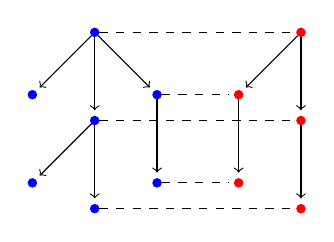
\begin{tikzpicture}[%
        every node/.style={circle,minimum size=3pt,minimum height=3pt, inner sep=0pt},
        shorten >=2pt,
        node distance=1cm
      ]
      \node [draw] (0) [color=blue, fill] {};
      \node [draw] (1) [color=blue, fill, below left=of 0] {};
      \node [draw] (2) [color=blue, fill, below=of 0] {};
      \node [draw] (3) [color=blue, fill, below right=of 0] {};
      \node [draw] (4) [color=blue, fill, below left=of 2] {};
      \node [draw] (5) [color=blue, fill, below=of 2] {};
      \node [draw] (6) [color=blue, fill, below=of 3] {};
      \node [draw] (7) [color=red, fill, right=of 0, xshift=1.5cm] {};
      \node [draw] (8) [color=red, fill, below left=of 7] {};
      \node [draw] (9) [color=red, fill, below=of 7] {};
      \node [draw] (10) [color=red, fill, below=of 8] {};
      \node [draw] (11) [color=red, fill, below=of 9] {};
      \path [draw] (0) edge[->]  node {} (1)
      (0) edge[->]  node {} (2)
      (0) edge[->]  node {} (3)
      (2) edge[->]  node {} (4)
      (2) edge[->]  node {} (5)
      (3) edge[->]  node {} (6)
      (7) edge[->]  node {} (8)
      (7) edge[->]  node {} (9)
      (8) edge[->]  node {} (10)
      (9) edge[->]  node {} (11);
      \draw[dashed] (0) -- (7);
      \draw[dashed] (3) -- (8);
      \draw[dashed] (2) -- (9);
      \draw[dashed] (5) -- (11);
      \draw[dashed] (6) -- (10);
    \end{tikzpicture}
    \label{fig:backward}
  \end{figure}
}

\def\forward{
  \begin{figure}
    \centering
    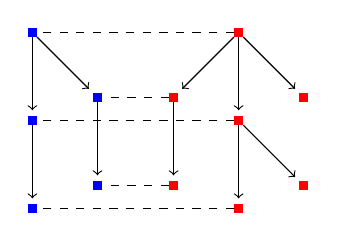
\begin{tikzpicture}[%
        every node/.style={rectangle,minimum size=3pt,minimum height=3pt, inner sep=0pt},
        shorten >=2pt,
        node distance=1cm
      ]
      \node [draw] (0) [color=red, fill] {};
      \node [draw] (1) [color=red, fill, below right=of 0] {};
      \node [draw] (2) [color=red, fill, below=of 0] {};
      \node [draw] (3) [color=red, fill, below left=of 0] {};
      \node [draw] (4) [color=red, fill, below right=of 2] {};
      \node [draw] (5) [color=red, fill, below=of 2] {};
      \node [draw] (6) [color=red, fill, below=of 3] {};
      \node [draw] (7) [color=blue, fill, left=of 0, xshift=-1.5cm] {};
      \node [draw] (8) [color=blue, fill, below right=of 7] {};
      \node [draw] (9) [color=blue, fill, below=of 7] {};
      \node [draw] (10) [color=blue, fill, below=of 8] {};
      \node [draw] (11) [color=blue, fill, below=of 9] {};
      \path [draw] (0) edge[->]  node {} (1)
      (0) edge[->]  node {} (2)
      (0) edge[->]  node {} (3)
      (2) edge[->]  node {} (4)
      (2) edge[->]  node {} (5)
      (3) edge[->]  node {} (6)
      (7) edge[->]  node {} (8)
      (7) edge[->]  node {} (9)
      (8) edge[->]  node {} (10)
      (9) edge[->]  node {} (11);
      \draw[dashed] (0) -- (7);
      \draw[dashed] (3) -- (8);
      \draw[dashed] (2) -- (9);
      \draw[dashed] (5) -- (11);
      \draw[dashed] (6) -- (10);
    \end{tikzpicture}
    \label{fig:forward}
  \end{figure}
}

\def\mixed{
  \begin{figure}
    \centering
    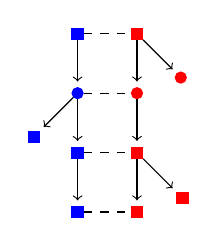
\begin{tikzpicture}[%
        every node/.style={rectangle,minimum size=4pt,minimum height=4pt, inner sep=0pt},
        shorten >=2pt,
        node distance=0.6cm
      ]
      \node [draw] (0) [color=blue, fill] {};
      \node [draw] (1) [circle, color=blue, fill, below=of 0] {};
      \node [draw] (2) [color=blue, fill, below left=of 1] {};
      \node [draw] (3) [color=blue, fill, below=of 1] {};
      \node [draw] (4) [color=blue, fill, below=of 3] {};
      \node [draw] (5) [color=red, fill, right=of 0] {};
      \node [draw] (6) [circle, color=red, fill, below=of 5] {};
      \node [draw] (7) [circle, color=red, fill, below right=of 5] {};
      \node [draw] (8) [color=red, fill, below=of 6] {};
      \node [draw] (9) [color=red, fill, below=of 8] {};
      \node [draw] (10) [color=red, fill, below right=of 8] {};
      \path [draw] (0) edge[->]  node {} (1)
      (1) edge[->]  node {} (2)
      (1) edge[->]  node {} (3)
      (3) edge[->]  node {} (4)
      (5) edge[->]  node {} (6)
      (5) edge[->]  node {} (7)
      (6) edge[->]  node {} (8)
      (8) edge[->]  node {} (9)
      (8) edge[->]  node {} (10);
      \draw[dashed] (0) -- (5);
      \draw[dashed] (1) -- (6);
      \draw[dashed] (3) -- (8);
      \draw[dashed] (4) -- (9);
    \end{tikzpicture}
    \label{fig:mixed}
  \end{figure}
}

\subsection{Memory Update}
\begin{frame}{\subsecname}

  \begin{block}{Updating the definition of the memory}
    \begin{itemize}
    \item Add a map \texttt{mem\_concrete: block -> Option Z}.
    \item Remember the size of blocks at allocation.
    \item Address-wise permissions.
    \end{itemize}
  \end{block}
  \vfill
  \begin{block}{Abstract Analysis}
    The stack block can be accessible if it is concrete.
  \end{block}
    \vfill
    \begin{exampleblock}{Proofs}
      \begin{itemize}
      \item Every memory operation preserves memory consistency.
      \item Abstract analysis is sound.
      \end{itemize}
  \end{exampleblock}

  
\end{frame}

\subsection{Memory Injection}
\begin{frame}{\subsecname}

  \begin{block}{Memory Injection}
    A map from some blocks of the source memory to blocks of the target memory.
  \end{block}
  \vfill
  \begin{block}{Changes}
    \begin{itemize}
    \item Concrete blocks mapped to concrete blocks, at the same address.
    \item No concrete private source blocks.
    \end{itemize}
  \end{block}
  \vfill
  \begin{exampleblock}{Proofs}
    Every memory operation preserves memory injection.
  \end{exampleblock}
  
\end{frame}

\subsection{Capture Semantics}
\begin{frame}{\subsecname}

  \comment{example}\\
  \comment{In Clight}

\end{frame}

\subsection{Mixed Simulations}
\begin{frame}{Proving the correctness of CompCert}
  \begin{block}{SmallStep Semantics}
    A relation between states (memory, program counter\dots).
  \end{block}
  \vfill
  \begin{columns}[T] % align columns
    \begin{column}{.48\textwidth}
      \begin{block}{Forward Simulation}
        Step in source $\rightarrow$\\ Matching step in target\\
        {\color{blue}Source\hfill\color{red}Target}
        \forward
      \end{block}
    \end{column}%
    \hfill%
    \begin{column}{.48\textwidth}
      \begin{block}{Backward Simulation}
        Step in target $\rightarrow$\\ Matching step in source\\
        {\color{blue}Source\hfill\color{red}Target}
        \backward
      \end{block}
    \end{column}%
  \end{columns}
\end{frame}

\begin{frame}{Changing the correctness proof}
  \begin{exampleblock}{Goal}
    A backward simulation between C and ASM.
  \end{exampleblock}
  \vfill
  \begin{alertblock}{Previous proof}
    Determinacy + forward simulation $\rightarrow$ backward simulation.\\
    No more determinacy!
  \end{alertblock}
  \vfill
  \begin{exampleblock}{Handling non-deterministic behavior}
    Non-deterministic behavior only for unknown external calls or builtin functions (capture).\\
    For every other state, we still have local determinism.
  \end{exampleblock}
\end{frame}

\begin{frame}{Mixed Simulations}
  \begin{block}{Mixed Simulation}
    External state ($\bigcirc$): Local backward simulation.\\
    Internal state ($\Box$): Local forward simulation.\\
    {\color{blue}Source\hfill\color{red}Target}
    \vspace{-0.8cm}
    \mixed
  \end{block}
  \vfill
  \begin{block}{Theorem}
    MixedSim (A,B) $\rightarrow$ BackwardSim ((atomic A),B).
  \end{block}
\end{frame}

\begin{frame}{The previous correctness proof}
  \oldprooffwds
  \vfill
  \begin{block}{Theorem}
    Forward Simulation Composition.
  \end{block}
\end{frame}

\begin{frame}{The previous correctness proof}
  \oldprooffwd
  \vfill
  \begin{block}{Theorems}
  \begin{itemize}
    \item ForwardSim(A,B) $\rightarrow$ BackwardSim(atomic(A),B).
    \item BackwardSim(A,B) $\rightarrow$ BackwardSim(A,atomic(B)).
  \end{itemize}
  \end{block}
\end{frame}

\begin{frame}{The previous correctness proof}
  \oldprooffactorbwd
  \vfill
  \begin{block}{Theorem}
    Backward Simulation Composition.
  \end{block}
\end{frame}

\begin{frame}{The previous correctness proof}
  \oldprooffinal
\end{frame}

\begin{frame}{The new correctness proof}
  \proofmixed
  \vfill
  \begin{block}{Theorem}
    MixedSim (A,B) $\rightarrow$ BackwardSim ((atomic A),B).
  \end{block}
\end{frame}

\begin{frame}{The new correctness proof}
  \proofmixedbwd
  \vfill
  \begin{block}{Theorem}
    BackwardSim(A,B) $\rightarrow$ BackwardSim(A,atomic(B)).
  \end{block}
\end{frame}

\begin{frame}{The new correctness proof}
  \proofatbwd
  \vfill
  \begin{block}{Theorem}
    Backward Simulation Composition.
  \end{block}
\end{frame}

\begin{frame}{The new correctness proof}
  \prooffinal
\end{frame}



\section{Evaluation}
\outline
\begin{frame}{\secname: Correctness}

  \begin{alertblock}{Admitted Theorems}
    Most mixed simulations.
  \end{alertblock}
  \vfill
  \begin{exampleblock}{Finishing the proofs}
    Two mixed simulations finished. Others should be very similar.
  \end{exampleblock}
  \vfill
  \begin{alertblock}{Casts semantics not fully implemented}
    We can still see the capture, and compile some C programs.
  \end{alertblock}
  
\end{frame}

\begin{frame}{\secname: Optimizations}
  \begin{tabular}{l c r}
    \lstinputlisting[linewidth=4cm]{listings/evallogical.c} &
    $\longrightarrow$ &
    \lstinputlisting[linewidth=6cm]{listings/evallogicalopt.c}
  \end{tabular}
  \vfill
  \hrulefill
  \vfill
  \begin{tabular}{l c r}
    \lstinputlisting[linewidth=4cm]{listings/evalconcrete.c} &
    $\longrightarrow$ & 
    \lstinputlisting[linewidth=6.5cm]{listings/evalconcreteopt.c}
  \end{tabular}

\end{frame}


\section{Conclusion}
\begin{frame}{\secname}

  \begin{exampleblock}{Results}
    \begin{itemize}
    \item The new memory model has been implemented in CompCert.
    \item It successfully gives semantics to Integer-Pointer casts.
    \item It allows optimizations.
    \item The proof of correctness is almost finished.
    \end{itemize}
  \end{exampleblock}
  \vfill
  \begin{block}{Future Work}
    \begin{itemize}
    \item Finish the mixed simulations proofs.
    \item Finish implementation of the integer-pointer cast semantics.
    \end{itemize}
  \end{block}
  
\end{frame}


\begin{frame}{}
  %last takeaway frame
  \begin{center}
  \begin{figure}
  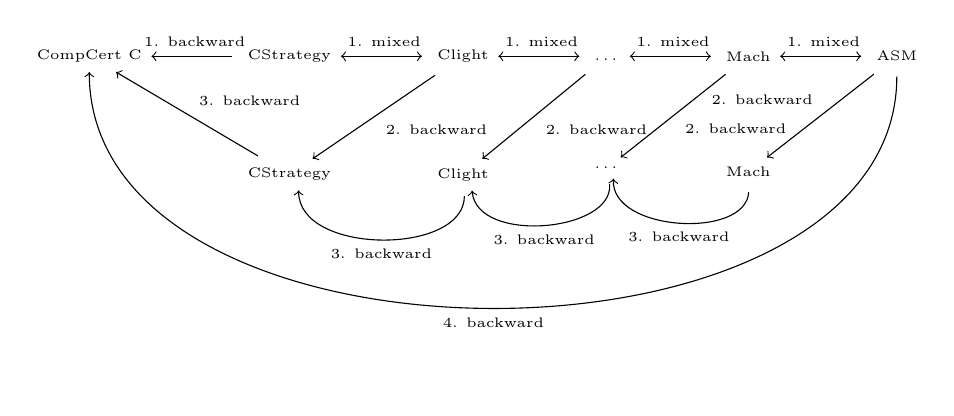
\begin{tikzpicture}[%
      every node/.style={rectangle, font=\tiny},
      shorten >=2pt,
      node distance=1.1cm
    ]
    \node (cc) [] {CompCert C};
    \node (cstrat) [right=of cc] {CStrategy};
    \node (clight) [right=of cstrat] {Clight};
    \node (dots) [right=of clight] {\dots\vphantom{C}};
    \node (mach) [right=of dots] {Mach};
    \node (asm) [right=of mach] {ASM};
    \node (atcstrat) [below=of cstrat] {\at{CStrategy}};
    \node (atclight) [below=of clight] {\at{Clight}};
    \node (atdots) [below=of dots] {\at{\dots}};
    \node (atmach) [below=of mach] {\at{Mach}};
    \path [draw] (cc) edge[<-, above] node {1. backward} (cstrat);
    \path [draw] (cstrat) edge[<->, above] node {1. mixed} (clight);
    \path [draw] (clight) edge[<->, above] node {1. mixed} (dots);
    \path [draw] (dots) edge[<->, above] node {1. mixed} (mach);
    \path [draw] (mach) edge[<->, above] node {1. mixed} (asm);
    \path [draw] (atcstrat) edge[<-,below right] node {2. backward} (clight);
    \path [draw] (atclight) edge[<-,below right] node {2. backward} (dots);
    \path [draw] (atdots) edge[<-,below right] node {2. backward} (mach);
    \path [draw] (atmach) edge[<-,above left] node {2. backward} (asm);
    \path [draw] (cc) edge[<-,above right] node {3. backward} (atcstrat);
    \path [draw] (atcstrat.300) edge[<-, bend right=90, below] node {3. backward} (atclight);
    \path [draw] (atclight.300) edge[<-, bend right=90, below] node {3. backward} (atdots);
    \path [draw] (atdots.300) edge[<-, bend right = 90, below] node {3. backward} (atmach);
    \path [draw] (cc) edge[<-, bend right=90, below] node {4. backward} (asm);
  \end{tikzpicture}
  \end{figure}
  \end{center}
\end{frame}


\end{document}
